%\section{Convolutional side-outputs for image segmentation}
\section{Side-outputs merging strategies and mathematical morphology post-processing}
\label{sec:method}

\begin{figure*}[!t]
\centering
\subfloat[Stage Layer Outputs (SLO)]{\resizebox{\textwidth}{!}{%
\begin{tikzpicture}[
std/.style={
  draw,
  text width=1.5cm,
  align=center,
  font=\strut\sffamily
  },
rnd/.style={
  draw=#1,
  rounded corners=8pt,
  line width=1pt,
  align=center,
  text width=2cm,
  minimum height=1cm,
  font=\strut\sffamily
  },
vac/.style={
  text width=2.5cm,
  align=center,
  font=\strut\sffamily
  },
ar/.style={
  ->,
  >=latex
  },
node distance=0.5cm and .5cm    
]



%The nodes for the left
\node[rnd] (inp)
  {Input layer};
\node[rnd=gruen_4b,right=of inp] (conv1)
  {Convolution};  
\node[rnd=gruen_4b,right=of conv1] (conv2)
  {Convolution};  
\node[draw,dashed,gruen_4b,inner sep=8pt,fit={(conv1) (conv2)}]
  (fit) {};
\node[rnd,right=1cm of conv2] (pool1)
  {Pooling};
\node[vac,left=-1cm of pool1, yshift=-1.5cm] (h1)
  {$\mathcal{H}_1$}; 
\node[vac,gruen_4b,left=-1cm of conv2, yshift=1cm] (s1)
  {Stage 1};   
\node[vac,right=-1cm of pool1] (p)
  {$\mathbf{\cdots}$}; 
  
\node[rnd=gruen_4b,right=-.7cm of p] (conv3)
  {Convolution};  
\node[rnd=gruen_4b,right=of conv3] (conv4)
  {Convolution};  
\node[rnd=gruen_4b,right=of conv4] (conv5)
  {Convolution};    
\node[draw,dashed,gruen_4b,inner sep=8pt,fit={(conv3) (conv5)}]
  (fit2) {};
\node[rnd,right=1cm of conv5] (pool2)
  {Pooling};
\node[vac,left=-1cm of pool2, yshift=-1.5cm] (h2)
  {$\mathcal{H}_n$};
  \node[vac,gruen_4b,left=-3cm of conv4, yshift=1cm] (s2)
  {Stage $N$};   
\node[vac,right=-1cm of pool2] (p2)
  {$\mathbf{\cdots}$};   

%Aux  
\coordinate (aux1) at ( $ (conv2.east|-conv2.west)!0.6!(pool1.west) $ );
\coordinate (aux2) at ( $ (conv5.east|-conv5.west)!0.6!(pool2.west) $ );

\draw[ar]  (inp) -- (conv1); 
\draw[ar]  (conv1) -- (conv2); 
\draw[ar]  (conv2) -- (pool1); 
\draw[ar,left=-1cm of pool1, yshift=-1.5cm]  (aux1) -- (h1); 
\draw[ar]  (conv3) -- (conv4);
\draw[ar]  (conv4) -- (conv5); 
\draw[ar]  (conv5) -- (pool2); 
\draw[ar,left=-1cm of pool2, yshift=-1.5cm]  (aux2) -- (h2); 
\end{tikzpicture}%
} \label{fig:slo}}
\hfil
\subfloat[All Layers Outputs (ALO)]{\resizebox{\textwidth}{!}{%
\begin{tikzpicture}[
std/.style={
  draw,
  text width=1.5cm,
  align=center,
  font=\strut\sffamily
  },
rnd/.style={
  draw=#1,
  rounded corners=8pt,
  line width=1pt,
  align=center,
  text width=2cm,
  minimum height=1cm,
  font=\strut\sffamily
  },
vac/.style={
  text width=2.5cm,
  align=center,
  font=\strut\sffamily
  },
ar/.style={
  ->,
  >=latex
  },
node distance=0.5cm and .5cm    
]



%The nodes for the left
\node[rnd] (inp)
  {Input layer};
\node[rnd=lila_10b,right=of inp] (conv1)
  {Convolution};  
\node[rnd=lila_10b,right=of conv1] (conv2)
  {Convolution};  
\node[rnd,right=1cm of conv2] (pool1)
  {Pooling};
\node[vac,right=-1cm of pool1] (p)
  {$\mathbf{\cdots}$}; 
  
\node[rnd=lila_10b,right=-.7cm of p] (conv3)
  {Convolution};  
\node[rnd=lila_10b,right=of conv3] (conv4)
  {Convolution};  
\node[rnd=lila_10b,right=of conv4] (conv5)
  {Convolution};    
\node[rnd,right=1cm of conv5] (pool2)
  {Pooling};
\node[vac,right=-1cm of pool2] (p2)
  {$\mathbf{\cdots}$};   

\node[vac,left=-1cm of conv2, yshift=-1.5cm] (h1)
  {$\mathcal{H}_1$};
\node[vac,left=-1cm of pool1, yshift=-1.5cm] (h2)
  {$\mathcal{H}_2$};    
\node[vac,left=-1cm of conv4, yshift=-1.5cm] (h3)
  {$\mathcal{H}_{n-2}$};
\node[vac,left=-1cm of conv5, yshift=-1.5cm] (h4)
  {$\mathcal{H}_{n-1}$};
\node[vac,left=-1cm of pool2, yshift=-1.5cm] (h5)
  {$\mathcal{H}_n$};


%Aux  
\coordinate (aux1) at ( $ (conv1.east|-conv1.west)!0.3!(conv2.west) $ );
\coordinate (aux2) at ( $ (conv2.east|-conv2.west)!0.6!(pool1.west) $ );
\coordinate (aux3) at ( $ (conv3.east|-conv3.west)!0.3!(conv4.west) $ );
\coordinate (aux4) at ( $ (conv4.east|-conv4.west)!0.3!(conv5.west) $ );
\coordinate (aux5) at ( $ (conv5.east|-conv5.west)!0.6!(pool2.west) $ );

\draw[ar]  (inp) -- (conv1); 
\draw[ar]  (conv1) -- (conv2); 
\draw[ar]  (conv2) -- (pool1); 
\draw[ar]  (conv3) -- (conv4);
\draw[ar]  (conv4) -- (conv5); 
\draw[ar]  (conv5) -- (pool2); 

\draw[ar,left=-1cm of pool1, yshift=-1.5cm]  (aux1) -- (h1);
\draw[ar,left=-1cm of pool2, yshift=-1.5cm]  (aux2) -- (h2); 
\draw[ar,left=-1cm of pool2, yshift=-1.5cm]  (aux3) -- (h3);
\draw[ar,left=-1cm of pool2, yshift=-1.5cm]  (aux4) -- (h4);
\draw[ar,left=-1cm of pool2, yshift=-1.5cm]  (aux5) -- (h5);   

\end{tikzpicture}%
} \label{fig:alo}}
\caption{Illustration for the two side-outputs extraction strategies:  (a) side-outputs extracted at each stage of the network and (b) side-outputs extracted at each convolutional layer}
\label{fig:extraction}
\end{figure*}

Hierarchies are long associated with the image segmentation task~\cite{jones97,cardelino06,najman12,xu16,cousty18}, to a degree that it improves a coherent organization of nested regions. The main motivation for using well-defined hierarchies is that different hierarchical level contains different detail level. In this work, instead of using a well-defined hand-engineered hierarchical structure, it is proposed to explore the concept abstraction resultant of the deep network dynamics, extracting side-outputs at different layers that ideally would contain different level of details. 


The idea is to combine the side-output maps into a single proposition to be evaluated in the image segmentation task, driving the learning flow towards creating adequate regions for the task. In an optimal scenario, the side-outputs would contain enough details to cope with the task and create coherent region proposals. 
%\remEwai{what mean whilst here? task=image segmentation = creation of coherent regions ?}

Amongst the many strategies for deep models, convolutional networks are well-known for the concept abstraction resulting from the multiple stages of convolution and have been successfully used for the object recognition task. They are usually composed of multiple layers, each layer being characterized by three nested functions, namely: (i) convolution; (ii) spatial pooling; and (iii) non-linear activation. 

Let $\mathbf{X}$ be a set of $N$ input images $I$. Formally, let a convolutional network $\mathit{f}$ composed by $L$ layers be defined as:

%\remEwai{$X$ should be defined} \remFeli{Done}
\begin{equation}
\mathit{f}(\mathbf{X})=\mathbf{W}_L\mathbf{H}_{L-1}
\end{equation}
\noindent in which:
\begin{itemize}
\item $\mathbf{W}_l$ is the associated weights for the layer $l$;
\item $\mathbf{H}_l$ is the output of the layer $l$, defined as
\end{itemize}

\small
\begin{equation}
\mathbf{H}_l= pooling(activation(\mathbf{W}_l\mathbf{H}_{l-1}))~\forall l \in \{1,...,L-1\}
\end{equation}
\normalsize
\noindent For consistency, consider $\mathbf{H}_0=\mathbf{X}=\{X_1, X_2,...,X_N\}$. %the set of $N$ input images $I$.

The VGG network~\cite{simonyan2014} is one of the first attempts to create deeper models following the convolutional scheme. The core of the layers in VGG is defined by a convolution $C$ immediately followed by a rectified linear unit, as follows:

%\remEwai{define $C_l$} \remFeli{Done}

\begin{equation}
C_l=ReLU(\mathbf{W}_{l}\mathbf{H}_{l-1})~\forall l \in \{1,..,L-1\}
\end{equation}
\noindent in which $ReLU(\cdot)=max(0,\cdot)$. There is also two types of stages, $\mathit{S}^{(1)}$ and $\mathit{S}^{(2)}$, that could formally defined as:
\small
\begin{align}
\mathit{S}^{(1)}&=ReLU(\mathbf{W}_l(ReLU(\mathbf{W}_{l-1}\mathbf{H}_{l-2})))\\
\mathit{S}^{(2)}&=ReLU(\mathbf{W}_l(ReLU(\mathbf{W}_{l-1}(ReLU(\mathbf{W}_{l-2}\mathbf{H}_{l-3})))
\end{align}
\normalsize
\noindent The output of a hidden layer is computed as $maxpool(\mathit{S}^{(1)})$ or $maxpool(\mathit{S}^{(2)})$ for all $S$ stages in the network.

Questions on which and how many side-outputs would be adequate for the image segmentation task are assessed using two different extraction strategies, both applied in the VGG network. Namely: (i) Stage Layer Outputs~(\textbf{SLO}), inspired by the HED model, creating one side-output for each VGG stage; and (ii) All Layers Outputs~(\textbf{ALO}), inspired by the RCF model, creating one side-output for each convolutional layer. 

Formally, the set $\mathcal{H}$ of $M$ side-outputs maps in each strategy is defined as:
\small
\begin{align}
\mathcal{H}_{SLO}=\{\mathcal{H}_1,...,\mathcal{H}_m|& m\in[1,S]~\text{and}~\mathcal{H}_m \in\{S^{(1)},S^{(2)}\}\}\\
\mathcal{H}_{ALO}=\{\mathcal{H}_1,...,\mathcal{H}_m|& m\in[1,L-1]~\text{and}~\nonumber\\&{H}_m=C_l~\forall l \in \{1,..,L-1\}\}
\end{align}
\normalsize

In the case of \textbf{SLO}, the number of side-outputs corresponds to the number of pooling layers in the network and for \textbf{ALO}, it is equal to the number of convolutional layers. An illustration for both strategies is presented in Figure~\ref{fig:extraction}.

\subsection{Merging strategies}
\label{ssec:mergin_strategies}
%\remEwai{a subsection cannot live alone :)} \remFeli{Done}

When dealing with side-outputs in convolutional networks, the main question is how to combine them, considering that they are presented in different scales and could represent different concepts. The goal is to produce a single proposition to be evaluated in the task, while retaining the useful information contained at different layers.

In this work, the strategy to overcome those challenges is to combine the side-outputs by exploring the knowledge of the learning process. To achieve that, it is proposed to apply simple merging functions that would enhance different desirable behavior, as described in the following: 
\begin{itemize}
\item \textit{ADD}: Aims to balance negative and positive weights;
\item \textit{AVG}: Aims to create a proposition representing the whole network learning;  
\item \textit{MAX}: Aims to represent confident values. 
\end{itemize}  

Formally, the single proposition $Z$ to be evaluated in the task, under each strategy could be defined as:

\begin{align}
Z_{ADD} &= \sum_{i=1}^{M}(\mathcal{H}_i)\\
Z_{AVG} &= \frac{\sum_{i=1}^{M}(\mathcal{H}_i)}{M}\\
Z_{MAX} &= \max_{1 \leq i \leq M} (\mathcal{H}_i)
\end{align} 

The operations are performed element-wise on each side-output. To cope with the different sizes presented at different layers, the side-output maps are first re-scaled to the input image size using a transposed convolution layer~\cite{dumoulin2016}, also called as ``deconvolutional layer''. In this process, the transposed weighted map is used to convolve the side-output maps with an appropriate kernel to up-sample each position while maintaining the connectivity pattern. After element-wise combination, a convolutional $1x1$ operation is performed with Relu activation, as Figure \ref{fig:side_outputs_method}.

\begin{figure}
  \caption{\color{red}Side ouputs. Image must be improved!}
  \centering
  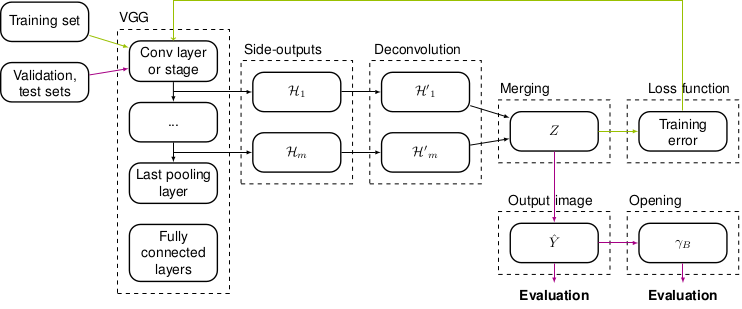
\includegraphics[width=1.\columnwidth]{figures/falreis/side_outputs_method.png}
  \label{fig:side_outputs_method}
\end{figure}

Once the combined map is created, it is evaluated on the segmentation task which aims to provide partition of an image into a set of regions representing meaningful areas. This could be reduced to a binary problem aiming to distinguish each pixel of the image as belonging to a region of interest or the background. If confronted with multiple regions of interest this minimal formulation could be executed individually and paired later. After pixel-wise evaluation for a single image, the following step is evaluate the accuracy for set of $N$ images.

%Considering once again the set of $N$ training images $\mathbf{X}$ and alike $\mathbf{Y}=\{Y_1, Y_2,...,Y_N\}$ the set of ground-truth images in which each pixel is labeled. The ground-truth images are used to calculate the pixel accuracy measuring the number of true positive pixels over the sum of true positive and negative pixels. The averg
%Accuracy = True Positive / (True Positive+True Negative)*100.

%. Each one of this images   Let $Z$ be the merged map obtained using one of the proposed functions and $|Z| = |I|, \forall I\in \mathbf{X}$.
%
%$\mathit{S}=\{(\mathit{X_n,Y_n}), \mathit{n}=1,...,\mathit{N}\}$ be the training input set for the network, in which $\mathit{X_n}$ is a set of $\mathit{N}$ images with three color channels and $\mathit{Y_n}$ the set of $\mathit{N}$ labels associated with each image with values belonging to $\{0,1\}$. Consider also $\mathbf{W}$ the layer set of parameters in which
%$\mathbf{w}=\{\mathbf{w}_1,...,\mathbf{w}_M\}$ is the associated weights for each one of the $\mathit{M}$ side output maps. The objective function for training the weights for the $\ell_{side}$ image map could be defined as:
%\begin{equation}
%\mathcal{L}(\mathbf{W},\mathbf{w})=\sum_{m=1}^M\alpha_m\ell_{side}^{(m)}(\mathbf{W},\mathbf{w}_m)
%\end{equation}

\subsection{Post-processing}
\label{ssec:post_processing}
%\remEwai{Maybe to short to be a section} \remFeli{Now subsection}

Mathematical morphology is consistent with the non-linear image analysis, presenting solid theoretical foundation and idempotent functions. The formulations are presented in the complete lattice geometric space, in which the functions are performed considering whole sets operating over another whole set. In mathematical morphology, the operators are known a priori and defined using the sets of structuring elements, also know as kernels, used to perform non-linear operations and induce sub-spaces bounded by order filters~\cite{najman13}.

In this work, it is proposed to use mathematical morphology as post-processing step, meaning that this step is not inserted in the learning stage. The main goal is to better cope with the fundamental properties of a well-segmented image, particularly, region uniformity and continuity. To achieve that, it is proposed to use a function filter, called area opening, which tend to destroy the small, thin and conspicuous areas. In the opening operation, the size of the structuring element determines the analyses by opening holes near boundaries and removing objects that are relatively smaller than a threshold parameter.

Formally, let $\hat{Y}\in \mathbb{R}^2$ be the output of a testing image consistent with the representation created by the parameters learned in the network. Consider $B$ a structuring element and $\gamma_B$ the morphological opening produced by it. Consider also $\lambda$ the threshold parameter which will determine how small a certain area must be to be purged. In this case,  $\gamma_B \subseteq \gamma_\lambda$ if and only if $B$ is a finite union of connected components of area greater or equal to $\lambda$. This additional step could reduce possible noises on the final result and improve the accuracy on distinguishing the road from other objects presented on the image.
